\documentclass[a4paper,12pt]{article}
\usepackage[utf8]{inputenc}
\usepackage{rotating}
\usepackage{lscape}
\usepackage{amssymb,amsmath,amssymb}
\usepackage[stable]{footmisc}
\usepackage{lmodern}
\usepackage{libertine}
\usepackage[libertine]{newtxmath}
\usepackage{lstfiracode}
%\usepackage[scale=.95]{inconsolata}
\usepackage[authoryear]{natbib}
\usepackage{babelbib}
\usepackage{booktabs, makecell, longtable}
\usepackage[usenames,dvipsnames]{xcolor}
\definecolor{darkblue}{rgb}{0.0,0.0,0.55}
\setcitestyle{aysep={}} 
\usepackage{etoolbox}
\makeatletter
\patchcmd{\NAT@citex}
  {\@citea\NAT@hyper@{%
	 \NAT@nmfmt{\NAT@nm}%
	 \hyper@natlinkbreak{\NAT@aysep\NAT@spacechar}{\@citeb\@extra@b@citeb}%
	 \NAT@date}}
  {\@citea\NAT@nmfmt{\NAT@nm}%
   \NAT@aysep\NAT@spacechar\NAT@hyper@{\NAT@date}}{}{}
\patchcmd{\NAT@citex}
  {\@citea\NAT@hyper@{%
	 \NAT@nmfmt{\NAT@nm}%
	 \hyper@natlinkbreak{\NAT@spacechar\NAT@@open\if*#1*\else#1\NAT@spacechar\fi}%
   {\@citeb\@extra@b@citeb}%
	 \NAT@date}}
  {\@citea\NAT@nmfmt{\NAT@nm}%
   \NAT@spacechar\NAT@@open\if*#1*\else#1\NAT@spacechar\fi\NAT@hyper@{\NAT@date}}
  {}{}
\makeatother
\usepackage{setspace}
\usepackage[top=2.3cm,bottom=2.3cm,left=2.4cm,right=2.4cm]{geometry}
\usepackage{graphicx}
\usepackage{dcolumn}
\usepackage{float}
\floatplacement{figure}{H}
\usepackage{pgf}
\usepackage{tikz}
\usetikzlibrary{arrows}
\usetikzlibrary{positioning}
\usepackage{mathtools}
\usepackage{caption}
\usepackage[UKenglish]{babel}
\usepackage[UKenglish]{isodate}
\cleanlookdateon
\exhyphenpenalty=1000
\hyphenpenalty=1000
\widowpenalty=10000
\clubpenalty=1000
\onehalfspacing
\usepackage[backref,pagebackref]{hyperref}
\renewcommand*{\backref}[1]{}
\renewcommand*{\backrefalt}[4]{%
	\ifcase #1 (Not cited.)%
	\or        Cited on page~#2.%
	\else      Cited on pages~#2.%
	\fi}
\renewcommand{\backreftwosep}{ and~}
\renewcommand{\backreflastsep}{ and~}
	
\hypersetup{
  pdftitle={What Drives State-Sponsored Violence?: Evidence from
  Extreme Bounds Analysis and Ensemble Learning Models},
  pdfauthor={Danilo Freire and Gary Uzonyi},
  pdfkeywords={genocide, mass killings, random forest, state-sponsored violence},
  pdfborder={0 0 0},
  breaklinks=true,
  linkcolor=Mahogany,
  citecolor=Mahogany,
  urlcolor=darkblue,
  colorlinks=true}

\title{What Drives State-Sponsored Violence?: Evidence from Extreme Bounds
Analysis and Ensemble Learning Models\thanks{We thank Toke Aidt, Robert
McDonnell, Umberto Mignozzetti, David Skarbek, and Graham Denyer Willis for
their helpful suggestions and comments. All replication materials are available
at
\href{https://github.com/danilofreire/mass-killings-prediction}{\texttt{https://github.com/danilofreire/mass-killings-prediction}}.}}

\author{Danilo Freire\thanks{Postdoctoral Research Associate, The Political
	Theory Project, Brown University, 8 Fones Alley, Providence, RI 02912,
	\href{mailto:danilofreire@gmail.com}{\texttt{danilofreire@gmail.com}},
	\href{http://danilofreire.github.io}{\texttt{http://danilofreire.github.io}}.
	Corresponding author.} 
	\and 
	Gary Uzonyi\thanks{Assistant Professor,
	Department of Political Science; Research Fellow, Howard H. Baker Jr. Center
	for Public Policy, University of Tennessee, 1640 Cumberland Ave, Knoxville,
	TN 37996, \href{mailto:guzonyi@utk.edu}{\texttt{guzonyi@utk.edu}},
\href{https://sites.google.com/site/uzonyigary/}{\texttt{https://sites.google.com/site/uzonyigary}}.}}

\date{\today}

\begin{document}
\maketitle
	
\begin{abstract}
 \noindent
The literature on state-sponsored violence has grown significantly over the last decades. Although scholars have suggested a number of potential correlates of mass killings, it remains unclear whether the estimates are robust to different model specifications, or which variables accurately predict the onset of large-scale violence. We employ extreme bounds analysis and random forests to test the sensitivity of 40 variables on a sample of 177 countries from 1945 to 2013. The results help clear the brush around mass killings, as few variables in this literature are robust determinants of atrocity. However, support for an opportunity logic persists as greater constraints on a government limit its ability to employ barbarous tactics. It appears that the Conflict Trap applies to government atrocity. Atrocity breeds atrocity, while wealthy stable democracies tend to avoid episodes of mass killing.
	
 \vspace{.75cm}
 \noindent
 \textbf{Keywords}: extreme bounds analysis, genocide, mass killings, random forests, state-sponsored violence
	
 \vspace{.25cm}
 \noindent
 \textbf{JEL Classification}: C52, C53, D74, H56, K10
\end{abstract}
	
\newpage
	
\section{Introduction}
\label{sec:intro}
	
\doublespacing
	
Since the end of World War II, mass killings, genocides, and politicides have claimed over 34.5 million lives \citep{marshall2017pitf}.\footnote{Genocide and politicide are the attempted intentional destruction of communal or political groups, respectively \citep[see][]{harff1988toward}. Mass killing includes these atrocities, as well as attacks against civilians that result in at least 1,000 deaths but are not intended to destroy a particular group \citep[see][]{ulfelder2008assessing}. While some conflate the logic of these types of atrocities \citep[e.g.,][]{rummel1995democracy, valentino2004draining}, others claim genocide and politicide follow a different logic from other forms of government violence \citep{kalyvas2006logic,stanton2015regulating}. For discussion on these important differences in conceptualisation see \citep[]{straus2007second, finkel2012macro}} The international community has responded with an effort to prevent further state-sponsored mass murder by strengthening laws against war crimes, genocide, and crimes against humanity. Furthermore, the United Nations established a Special Adviser on the Prevention of Genocide and recognised its members' responsibility to protect civilian populations within and outside their own borders. Yet, such atrocities still occur. Recently, President al-Assad of Syria has massacred tens of thousands of civilians during the Syrian Civil War \citep{goldman2017nyt}. Similarly, South Sudan's President Kiir is actively starving and killing civilians from dissident and rival tribes \citep{nichols2017reuters}. While there is some evidence that such atrocities may be declining since the Cold War \citep{valentino2014we}, the international community has been far from successful in realising slogans like ``Never Again'' and ``Not on My Watch'' \citep{cheadle2007not}.
	
Ultimately, effective prevention requires us to understand why these atrocities occur. In this vein, the academic community has laboured tremendously to establish evidence-based theories as to why governments engage in brutality against their civilian populations. Indeed, since 1995, there have been over 45 quantitative political science articles focused on explaining government-sponsored killing of civilians. Overall, the mass violence literature agrees that government atrocity follows an opportunity logic: as threat increases, so does the likelihood of atrocity, if the costs to such violence are not prohibitive. However, there is little consensus on what factors influence the level of threat or costs a regime faces. Part of the reason for this uncertainty is that scholars use very different model specifications when testing their arguments, thus small changes in model parameters could influence the robustness of empirical results and the inferences we draw from these findings.
	
To overcome these limitations and provide a better understanding of government atrocity, we employ extreme bounds analysis and random forests to identify the most robust determinants of state-sponsored atrocities. Our approach is similar to \cite{hegre2006sensitivity} seminal analysis on the causes of civil war onset, but we provide additional tests to verify whether complex interactions and nonlinearities are driving the statistical results \citep{bell2015examining,jones2015exploratory,jones2018there,muchlinski2015comparing}. In conducting this analysis, we address three debates in the mass violence literature:
	
\begin{enumerate}
 \item Why do some governments engage in mass killings, genocides, or politicides? This is the primary question asked by activists, policymakers, and scholars in this field of research. 
 \item Does the logic underpinning government decision-making follow different patterns during peacetime and wartime? Recent research suggests that government atrocity occurs predominantly during periods of civil unrest \citep{harff2003no} which has led some scholars to restrict their analyses to only periods of civil war \citep[e.g.,][]{colaresi2008kill, valentino2004draining} or concentrate on predicting both the onset of civil war and atrocity \citep{goldsmith2013forecasting}. Yet, others estimate models of all country-years \citep[e.g.,][]{krain1997state, montalvo2008discrete}, raising questions of how well these studies speak to each other.
 \item Is there a difference in logic between those atrocities labelled as genocide or politicide, compared to other mass killings? While the Political Instability Task Force \citep{marshall2017pitf} provides the most widely used data on government atrocity, others provide data with much more lenient inclusion criteria \citep[e.g.,][]{stanton2015regulating, ulfelder2012forecasting}. These differences in definition of atrocity have led to divergent results, raising questions about important determinants of government behaviour \citep[for discussion, see][]{straus2007second, uzonyi2016domestic, wayman2010explaining}.
\end{enumerate}

Our analysis tests the sensitivity of 40 variables on a sample of 177 countries from 1945 to 2013. Our findings partially confirm previous research -- unstable countries are more likely to witness the regime employ atrocity \citep[e.g.,][]{goldsmith2013forecasting,harff2003no,krain1997state}. However, many of the factors scholars often cite as observable indicators of such instability -- regime transitions, coups d'état, the presence of militias, etc. -- are not good proxies for instability. Thus, policymakers may be looking for the incorrect signs of impending atrocity when seeking to prevent its onset. Furthermore, we find that the conclusions scholars draw regarding the likelihood of government atrocity largely depend on whether they combine peace and war years or just analyse periods of civil wars, as patterns in mass killings differ dramatically across these contexts. Lastly, we find that genocide and politicide follow vastly different patterns of onset than other forms of state-sponsored mass murder. This is further evidence that different logics govern different forms of political violence \citep{stanton2013terrorism}.

Overall, these findings raise concerns about policy options for preventing violence against civilians. If our conclusion is that unstable countries are violent, then preventing atrocity likely requires significant investments of time and resources in state-building, which is often politically and practically unfeasible \citep{doyle2006making}.  This analysis contributes significantly to the political violence literature by highlighting the parsimonious nature of the logic behind government atrocity and clearing away much of the empirical clutter surrounding this conclusion. 
	
\section{Empirical Methods}
\label{sec:methods}
	
To conduct our analysis, we began by surveying the quantitative political science literature on the causes of government mass killing since Rummel's (\citeyear{rummel1995democracy}) seminal work on the subject. Counting only published works, we identified 45 articles which employed logit or probit models of mass killing onset in a global sample.  We then included all variables that appeared in at least two of these papers in our data set at the country-year unit of analysis for all years from 1945 to 2013. The appendix provides a complete list of the articles we considered and a complete list of the variables we included in our models. Next, we estimated an extreme bounds analysis to determine which variables were the most robust in explaining the onset of government atrocity. Then, we estimated a distributed random forest analysis to see which of the variables best predicted the onset of these atrocities. In this section, we provide more detail on each of these estimation procedures before turning to the results of both analyses in the next section.

\subsection{Extreme Bounds Analysis}
\label{subsec:eba}

Th first method we employ to test the robustness of the potential determinants of state-led violence is the extreme bounds analysis (EBA). Researchers have employed EBA to assess the sensitivity of the determinants of civil war \citep{hegre2006sensitivity}, coups d'état \citep{gassebner2016expect}, democratisation \citep{gassebner2013extreme}, economic growth \citep{levine1992sensitivity, sala1997just}, nuclear deterrence \citep{bell2015examining}, and political repression \citep{hafner2005right}. The method is particularly useful when there is no consensus about which covariates belong in the ``true'' regression model \citep[178]{sala1997just} and scholars worry that omitted or unnecessary predictors can bias the model estimates \citep[60]{angrist2008mostly, clarke2005phantom, elwert2014endogenous, spector2011methodological}. 
More specifically, the main purpose of EBA is to estimate the distribution of coefficients of each predictor $x$ in an exhaustive combination of regression models with $y$ as a dependent variable. \cite[308]{leamer1985sensitivity} proposed that ``sturdy'' variables are those whose minimum and maximum of their coefficient distribution have the same sign and are situated at a distance from zero. If we are to use the conventional value of $p < 0.05$, the mean of the variable coefficients' distribution should be located at least $1.96$ standard deviations away from zero. 
	
Leamer's criterion is intuitive, but other authors contend it is too strict for most social science applications. \cite{sala1997just} argued that Leamer's EBA would increase the number of false negatives; in other words, it would classify as fragile covariates that are truly associated with the response. In this paper, we use Sala-i-Martin's \citeyear{sala1997just} more flexible version of EBA and consider the whole range of values of $CDF(0)$. We choose to use the whole distribution because the aggregate $CDF(0)$ allows us to move away from a binary indicator of robustness and present the estimations with their appropriate degrees of confidence. Our focus is the percentage of the variable's cumulative distribution function that is smaller or greater than zero. We do not assume that the CDFs are normally distributed and use Sala-i-Martin's generic model instead.\footnote{The generic model provides a better fit to our data. Histograms for all coefficients are available in online appendix.} We specify our models as follows:
	
\begin{equation}
\text{\textit{Mass Killing Onset}}_{it} = \beta_{M}M_{it} + \beta_{F}F_{it} + \beta_{Z}Z_{it} + v_{it}
\end{equation}
	
Our main dependent variable is \textit{Mass Killing Onset}, which denotes the onset of government-sponsored killings. \citet[2]{ulfelder2008assessing} define a mass killing as ``any event in which the actions of state agents result in the intentional death of at least 1,000 noncombatants from a discrete group in a period of sustained violence''. Respectively, $i$ and $t$ indicate country and year. $M$ is a set of three covariates that are included in every model due to their prominence in the literature \citep{levine1992vale}. In our analysis, $M$ includes the natural logarithm of the GDP per capita to control for income, the Polity IV index to control for level of democracy, and a linear time trend since the last episode of government-led atrocity to account for temporal dependence. $F$ denotes a vector of variables of interest, and $Z$ is a vector of other control variables in addition to those included in $M$. $v$ is the error term. In practice, however, since we are interested in the effect of all variables in the data set and do not have true control variables, except from $M$, $F$ and $Z$ are interchangeable. We thus only use this notation to help clarify the connection of our analysis to previous conflict scholars who employed similar extreme bounds analysis \citep[e.g.,][]{hegre2006sensitivity,gassebner2016expect}. Following \citet[514]{hegre2006sensitivity}, we lagged the independent variables one year to reduce the risk of endogeneity. 

Although our dependent variable is dichotomous, we use linear probability models in our main analysis. \citet[298]{gassebner2016expect} argue that linear probability models are less prone to convergence problems and their results can be readily interpreted. Since the data are grouped into countries, we also use cluster-robust standard errors.
	 
As a precaution against collinearity, we place a limit on the Variance Inflation Factor (\textit{VIF}) of all regression coefficients. The VIF estimates how much of the variance of each predictor is dependent on the other covariates in a model. A VIF of 1 indicates that the predictor is uncorrelated with the remaining covariates. VIF limits are often arbitrary \citep{bell2015examining,o2007caution}, thus here we use a moderately conservative VIF of 7. As robustness tests, we run the same models without restriction and with different cut-offs.
	
Two variables were omitted from EBA models but included in the machine learning estimations. The first is \textit{democracy}, a dummy variable that indicates whether the country has a Polity IV score equal or higher than 5. The second is \textit{interstate war}, a binary covariate measuring if the country is at war in a given year \citep{sarkees2010resort}. We have decided to omit democracy because of its evident correlation with the Polity measure and interstate war due to its correlation with our dependent variables. EBA models do not converge otherwise.\footnote{This is a typical case of multicollinearity and conceptual overlap. \citet{hlavac2016eba} suggests specifying a set of mutually exclusive variables to avoid the issue. However, as the Polity index is one of our core variables, we decided to drop the binary democracy indicator and use the continuous measure as it provides more details about the effect of political regimes on mass killings. More information available in the appendix.}  Since this problem does not affect machine learning algorithms, the two variables were included in the second set of estimations.
	
Lastly, we depart slightly from Sala-i-Martin's suggested method and do not assign weights to EBA. Although he recommends using goodness-of-fit measures to construct regression weights, we agree with \citet{sturm2002robust} and \citet[299]{gassebner2016expect} and use the unweighted version of the CDF instead. Goodness-of-fit indicators are not equivalent to the probability of a given model being true \citep{anscombe1973graphs,king1986not}, and the weights constructed this way are not invariant to transformations in the dependent variable. Moreover, our data set has a number of missing observations, so model comparison measures could be misleading \citep{lall2016multiple}.
	
\subsection{Random Forests}
\label{sub:drf}

We also make use of random forest (RF) \citep{breiman2001random} to evaluate whether the empirical results discussed in the mass killings literature are not driven by rigid parametric assumptions and model specifications. Random forest is a machine learning algorithm that consists of a combination of individual decision trees. In a classification problem, each decision tree uses a vector of covariates to split the dependent variable into two increasingly homogeneous parts \citep{breiman2001statistical}. However, decision trees are prone to overfitting, i.e., they match the original data set so closely that they tend to perform poorly with new data \citep{dietterich1995comparison,ho1998random}. Random forest, in contrast, avoids this issue by growing a decision tree only to a bootstrap sample of the original data, selecting random features at each split, then aggregating the different trees into a single prediction. If the independent variable is continuous, the algorithm will simply choose the average value of the predictions as the best candidate; if the covariate is discrete, the majority class will be employed. The simple procedure of leaving out some data points and growing separate trees with a random subset of covariates is sufficient to eliminate the risk of overfitting \citep[9-10]{jones2015exploratory}.
	
Random forest has many desirable properties, such as ``highly accurate predictions, robustness to noise and outliers, internally unbiased estimate of the generalisation error, efficient computation, and the ability to handle large dimensions and many predictors'' \citep[7]{muchlinski2015comparing}. Thus, random forest allows the researcher to estimate very flexible models with minimal assumptions. Unlike parametric methods such as ordinary least squares or logistic regressions, the analyst does not have to impose any distributional form to the data-generating process. As a result, random forest is able to effectively uncover complex, nonlinear interaction effects in the data without prespecification \citep{jones2015exploratory,jones2018there}.
	
In this paper we use distributed random forest (DRF) to model our data, a slightly modified version of the original random forest algorithm \citep{h2o2017}. The DRF has two additional features that are useful for our purposes. Firstly, DRF is optimised for big data, as it grows decision trees on separate cores to speed up computation time. Secondly, in DRF, non-observed cases are not assumed to be missing at random, but rather as values that contain information in themselves. The algorithm assumes that observations are missing for a reason, what is most likely the case with social science data \citep{lall2016multiple}. This is a more conservative approach than assuming that missing cases fit into an underlying parametric distribution.\footnote{For more information about how the distributed random forest algorithm deals with missing observations, please refer to: \href{http://docs.h2o.ai/h2o/latest-stable/h2o-docs/data-science/drf.html}{\texttt{http://docs.h2o.ai/h2o/latest-stable/h2o-docs/data-science/drf.html}} (access: December 2017).}
	
The DRF has a series of hyperparameters that can be tuned to improve its predictive performance. For instance, users can control the number of decision trees in each iteration, how deep trees should grow, and many other options. The interaction between parameters is generally complex and may involve thousands of potential combinations. As an example, a researcher interested in four parameters with 10 values each would have to estimate 10,000 models before deciding which is the most efficient one. Also, machine learning parameters are sensitive to the data at hand, that is, an optimal solution for one problem cannot be readily implemented in another data set \citep{genuer2008random,goldstein2010application,jones2015exploratory}.
	
To address these issues, we perform a grid search to select the most accurate random forest model \citep[123]{cook2017h2o}. We estimate a model for every possible combination of the hyperparameter space to make sure our results are robust to different specifications. For model selection, we follow the literature on predictive political science and use the area under the ROC curve (AUC) as our model evaluation metric \citep[e.g.,][]{hill2014empirical,ward2010perils,ward2013learning}. Models with higher AUC values are considered more accurate.
	
We add several parameters to the grid search. The first is the number of independent trees to grow in each forest. The starting values are 256, 512, and 1024 trees. The machine learning literature does not provide a heuristic on how large a random forest should be, but \citet[166]{oshiro2012many} affirm that ``from 128 trees there is no more significant difference between the forests using 256, 512, 1024, 2048 and 4096 trees.'' We employ a more conservative approach and start from a higher value that the authors suggest as adding more trees do not reduce prediction accuracy \citep[7]{breiman2001statistical}.
	
The depth of each decision tree also influences the algorithm performance. Deeper trees indicate more complex models, and in general they provide a better fit to the data. Nevertheless, this complexity comes at the risk of overfitting, so deeper trees are not necessarily the most adequate solution for every model \citep[596]{friedman2001greedy,segal2004machine}. In this article, we let the algorithm decide among using 10, 20, or 40 levels for each tree. 
	
We test whether having balanced classes of our dependent variable (mass killing onset) affects the predictive ability of the model. Since the response measure is heavily imbalanced, oversampling the positive responses could potentially improve our results \citep{chawla2004special,del2014use,japkowicz2002class}. 
We also vary how many variables should be considered for each split in the data. The default option is to use $\sqrt{p}$, where $p$ is the number of columns in the data set. As we have 40 covariates of interest, we have selected 5, 6 and 7 variables per split. The DRF uses a majority voting procedure to select which variable is most important. Additionally, the algorithm chooses the percentage of the training set to be modelled by each tree. The default option is 63.2\%, but we include the options of using 50\% and 100\% of the data. Similarly, we give a range of options for choosing how many columns will be included in each tree. The algorithm can randomly choose among 50\%, 90\% or 100\% of the independent variables when estimating a decision tree.

Finally, we use three types of histogram to find optimal split points for each independent variable. Decision trees consider every value of a given independent variable as a potential candidate for a split in the training data. This process is notably time-consuming, and computation time can be significantly reduced at little loss of precision by taking discrete values of the predictor distribution. The DRF algorithm also offers the choice of randomly cycling through all histogram types, including one type in each tree estimation. We adopt this ``round robin'' arrangement as it is both efficient and parsimonious.
	
\section{Results}
\label{sec:results}
	
We endeavour to answer three questions in our analysis: (1) what are the robust predictors of government mass killing, (2) do these predictors differ when considering only cases of civil war, and (3) are genocide and politicide different than other forms of atrocity? Table \ref{tab:eba01} summarises our main EBA results in answering Question 1. The table shows the average coefficient estimate of all regressions for each robust variable along with their mean standard deviations.\footnote{A list of all independent variables and coding rules are available in the appendix.} The table also displays the percentage of regressions that are statistically significant at the 90\% level. $CDF(0)$ represents the cumulative distribution function, which is the area of the distribution that falls above or below zero.\footnote{We show whichever area is the largest. The sign of the average $\beta$ coefficient indicates if most of the cumulative distribution is located above or below zero.} This is our main statistic of interest, and we consider a covariate to be robust if it has a $CDF(0)$ of 0.9 or higher \citep[181]{sala1997just}. Lastly, we report the number of estimated regressions models which included each variable.

\begin{table}[H]
\centering
\begin{tabular}{lrrrrr}
\hline
\textbf{Variable} & \textbf{Avg. $\beta$} & \textbf{Avg. SE} & \textbf{$\%$ Sig.} & \textbf{CDF(0)} & \textbf{Models} \\ \hline
\textit{Base variables} &  &  &  &  &  \\
Log GDP per capita & -0.0091 & 0.0052 & 76.055 & 0.9335 & 226707 \\
 &  &  &  &  &  \\
\textit{Additional variables} &  &  &  &  &  \\
Post-Cold War years & -0.0133 & 0.0085 & 72.845 & 0.9472 & 35614 \\
UCDP civil war onset & 0.0529 & 0.0321 & 52.378 & 0.9441 & 20854 \\
Previous riots & 0.0140 & 0.0100 & 56.242 & 0.9216 & 35614 \\
UCDP ongoing civil war & 0.0172 & 0.0115 & 65.652 & 0.9092 & 20854 \\
Ethnic diversity (ELF) & 0.0184 & 0.0137 & 56.674 & 0.9050 & 35614 \\
Polity IV squared & -0.0002 & 0.0001 & 61.206 & 0.9031 & 35614 \\ \hline
\end{tabular}
\caption{Extreme Bounds Analysis -- Mass Killings (Robust Variables Only)}
\label{tab:eba01}
\end{table}
	
Seven variables pass our EBA criteria and three of them decrease the likelihood of mass killings. First, as widely suggested in the literature, the natural logarithm of GDP per capita is negatively associated with the onset of mass killings \citep[e.g.,][]{besanccon2005relative, easterly2006development,esteban2015strategic}. Second, the post-Cold War years are correlated with lower levels of government violence. Indeed, this finding is in line with several studies that point to a general decline in violence over the last decades, including riots, civil wars, and urban crime \citep{pinker2011better,straus2012wars,valentino2014we}. The third robust variable is the squared term of the Polity IV political regime index. This finding points to a nonlinear relationship between political regime and mass killings, thus providing further evidence that democracy reduces state-sponsored violence \citep{rost2013will,rummel1995democracy} and that regimes that mix democratic with autocratic features have the highest risk of conflict \citep{hegre2001toward,muchlinski2014grievances}.
	
Four variables are robustly and positively associated with Ulfelder and Valentino's (\citeyear{ulfelder2008assessing}) indicator of government-sponsored violence. Onset and continuation of civil wars are correlated with mass killings, but only when we employ the UCDP measures of violent conflict. We find no effect for the variables compiled by the Correlates of War project or \cite{cederman2010ethnic}. Former instances of political turmoil also have a positive coefficient in our models. Moreover, countries with a previous history of riots are more prone to state violence, which suggests that government repression is path dependent \citep[e.g.,][]{gurr2000peoples,harff2003no,krain1997state,nyseth2017re}. Our results also show that higher levels of ethnic diversity increase the likelihood of atrocities against civilians. Nevertheless, ethnic diversity does not pass all additional tests we implement below and the sturdiness of this finding remains open to question.

Overall, the EBA indicates two patterns in answer to our first question on the causes of mass killing. Atrocity is (1) more likely when violence is already present, reducing the costs of escalating brutality and (2) is less likely as domestic and international constraints increase, increasing the costs of escalating violence further. These patterns support the dominant opportunity narrative in the literature. However, several of the variables commonly used to proxy opportunity, such as military size or regime change, are not robust predictors of atrocity. Thus, this analysis helps clear away much of the brush around the opportunity argument.

Figure \ref{fig:drfuv} presents the ten most important predictors of state-sponsored violence in our random forest models. Overall, the machine learning estimations have a good fit, with an AUC of about 0.83 in the validation sample. The algorithm confirms some of the main findings of EBA, yet they also show some interesting patterns. Only democracy and state capacity appear to be robust explanators of mass killing in both EBA and random forest models. These patterns further support the refrain that stable states tend to stay stable states. 

\begin{figure}[ht]
    \centering
    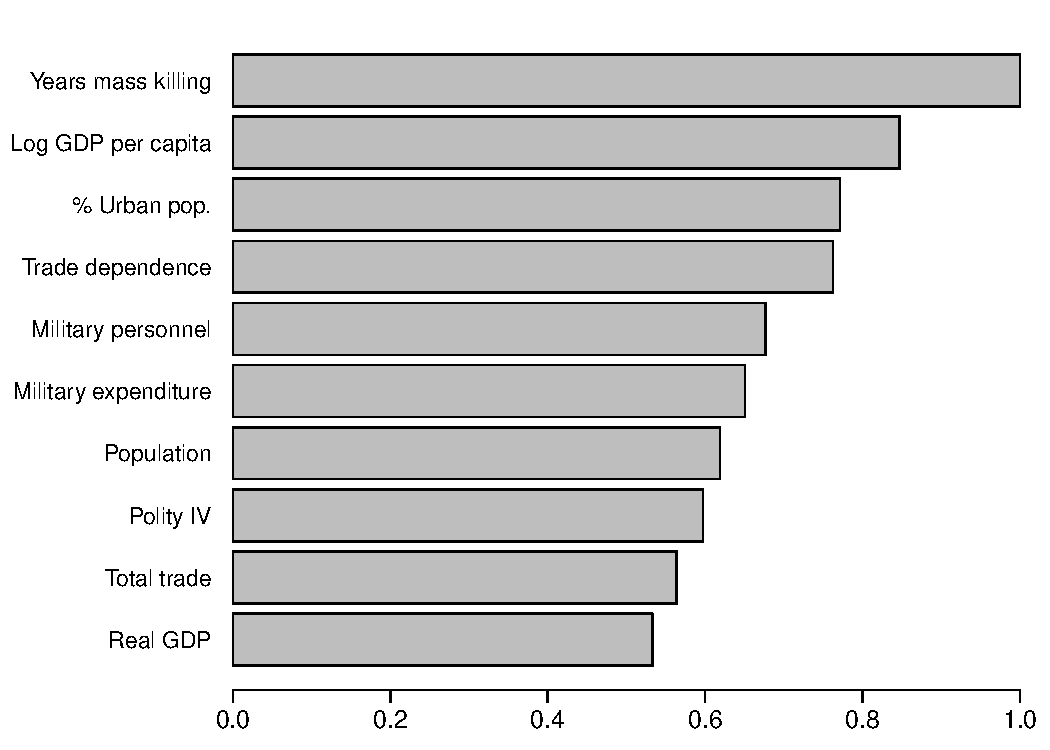
\includegraphics[width=.8\textwidth, height=8.25cm]{images/rf-mk.pdf}
    \caption{Distributed Random Forest -- Variable Importance (Scaled)}
    \label{fig:drfuv}
\end{figure}
	
Interestingly, several variables that are not robust explanators of mass killing in the EBA, have large importance in the machine learning estimates. Variables related to characteristics of the military forces are a good examples. As we see below, parametrisation and interactions likely account for this difference. The linear model imposes a parametric structure to the covariate, and the relationship between an independent variable and the response may be a nonlinear one. Also, variables can be relevant predictors only when in interaction with each other. In both cases, those relationships will be captured in the machine learning estimations but not in the extreme bounds analysis. 

% Moreover, one should have in mind that the EBA and DRF play two distinct, albeit complementary, academic goals: explanation and prediction \citep{bell2015examining,breiman2001statistical,ward2010perils}. In the first case, the main purpose is to understand historical patterns, the latter method tests the predictive power of the covariates using out-of-sample data. There is no reason to suspect the results obtained in the EBA, but the DRF provides a stricter test to the covariates as it uses data that the training model had not seen. This provides a better safeguard against overfitting and model mispecification.

Figure \ref{fig:drfdpp} displays the partial dependence plots for the ten variables that the distributed random forests highlight as the most important explanators of mass killing onset. These graphs are akin to marginal effect plots in correlation models and help clarify the directional effects of these variables over their entire range. For example, we are able to see that the effects of Years since Last Mass Killings and Polity IV are highly nonlinear, or that Log GDP per capita does not decrease the likelihood of mass killings after it reaches a value of 10.

\begin{figure}[H]
    \centering
    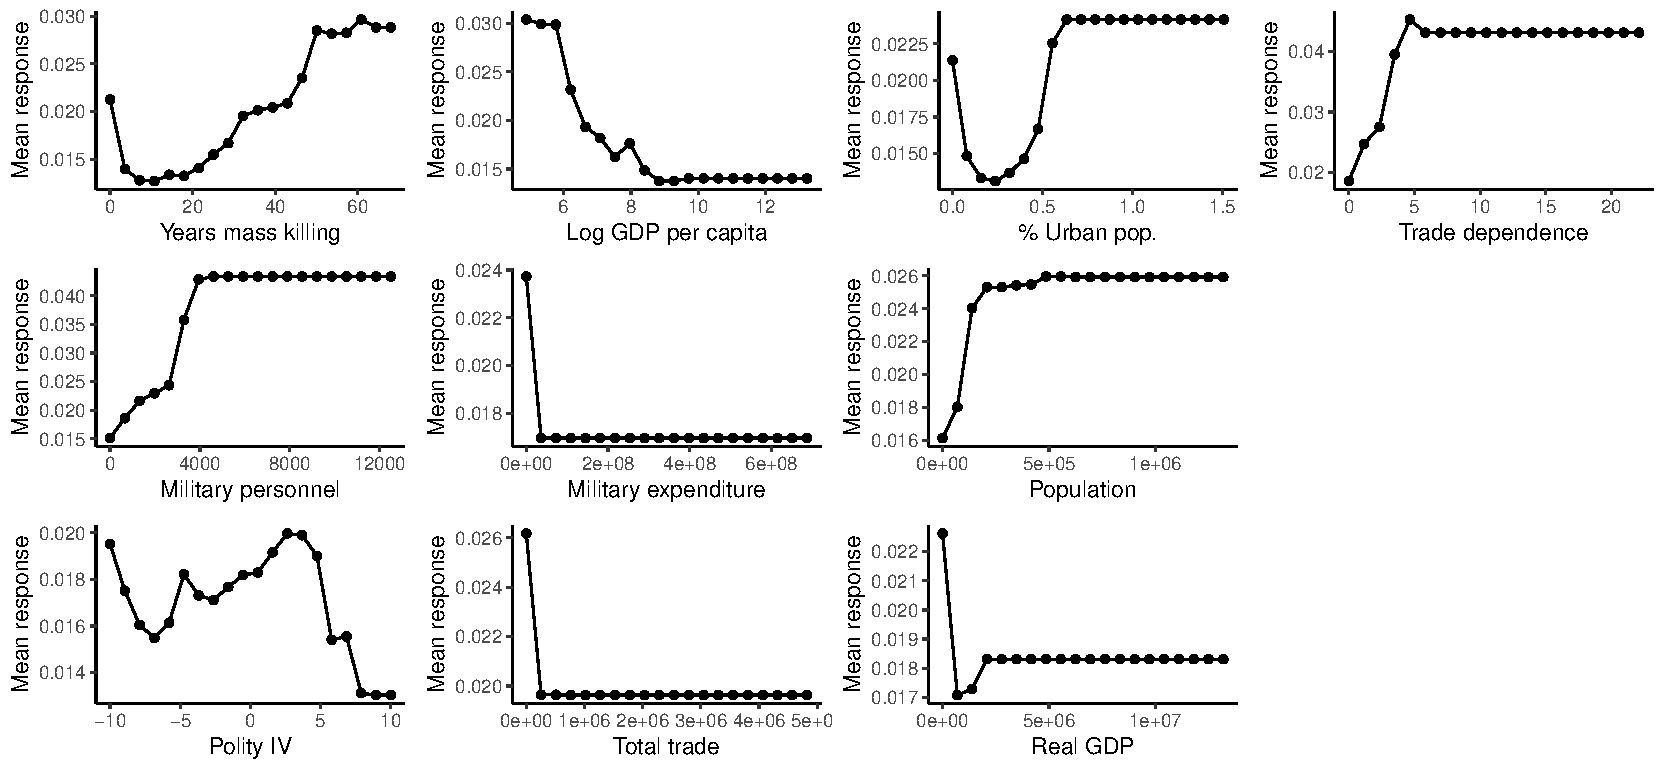
\includegraphics[width=\textwidth, height=8cm]{images/rf-mk-pd.pdf}
    \caption{Distributed Random Forest -- Partial Dependence Plots}
    \label{fig:drfdpp}
\end{figure}

% One paragraph on the results

Table \ref{tab:ucdp} presents our EBA results when we restrict our analysis to only civil war years to answer Question 2. We consider three different codings of civil war: (1) the Uppsala Conflict Database Program  (\citeyear{allansson2017organized,gleditsch2002armed}), (2) the Correlates of War project \citep{sarkees2010resort}, and (3) ethnic civil war from \citet{cederman2010ethnic}. We find two important patterns. First, considering only civil war years provides a very different understanding of atrocity. Across these models, the only similarity with the full analysis is that mass killing is less likely post-Cold War. Instead, military factors, such military size and militias, and territorial war aims are the most robust predictors of atrocity once war begins. However, contrary to past expectation \citep{koren2017means}, militias have a negative impact on the likelihood of mass killings. Second, there is wide variation in which variables are robust depending on how we code civil war. Across our three codings, no variable is robust to all codings and only territorial aims and militias are robust to more than one coding. These results are concerning for scholars using correlation models, as they indicate that our understanding of atrocity, from null hypothesis testing, is largely dependent on which coding of civil war we use. For example, only the UCDP data suggests that the post-Cold War years see less barbarism than during the Cold War.

\newpage

\begin{table}[H]
\centering
\begin{tabular}{lrrrrr}
\hline
\textbf{Variable} & \textbf{Avg. $\beta$} & \textbf{Avg. SE} & \textbf{$\%$ Sig.} & \textbf{CDF(0)} & \textbf{Models} \\ \hline
\textit{UCDP Data} &  &  &  &  &  \\
Territory aims & -0.044 & 0.019 & 74.997 & 0.9804 & 17902 \\
Post-Cold War years & -0.038 & 0.019 & 66.574 & 0.9222 & 17902 \\
 &  &  &  &  &  \\
\textit{COW Data} &  &  &  &  &  \\
Physical integrity & 0.024 & 0.013 & 66.674 & 0.9564 & 17902 \\
Militias & -0.099 & 0.048 & 73.104 & 0.9490 & 17902 \\
Years since last mass killing & 0.006 & 0.002 & 88.208 & 0.9472 & 101583 \\
Previous riots & 0.078 & 0.041 & 65.412 & 0.9348 & 17902 \\
Ethnic diversity (ELF) & 0.095 & 0.062 & 48.615 & 0.9000 & 17902 \\
& & & & \\
\textit{Cederman et al. Data} &  &  &  &  &  \\
Territory aims & -0.051 & 0.026 & 74.288 & 0.9167 & 17902 \\
Militias & -0.050 & 0.035 & 52.240 & 0.9101 & 17902 \\ \hline
\end{tabular}
\caption{EBA -- Mass Killings during Civil Wars (Robust Variables Only)}
\label{tab:ucdp}
\end{table}
	
When we analyse the three codings of civil war using our random forest analysis, we find further intricacies in the patterns of mass killing. First, the machine learning estimates highlight a different set of variables than the EBA when analysing the UCDP and Ethnic War data. However, the COW EBA and machine learning analyses both highlight the importance of human rights, previous riots, and the time since the state last engaged in mass killing. Thus, the COW analysis provides the most stable picture of atrocity during civil war. It again highlights the important pattern of the Conflict Trap: violence breeds violence. Second, though, the three codings of civil war each highlight a very similar set of strong predictors of atrocity during conflict. Therefore, the machine learning estimates are not as dependent on the data set employed as are the EBA results. This is good news for scholars of mass killing because it indicates that while our parametric models do not produce robust findings across different civil war data sets, our nonlinear models are able to given us a consistent and clear picture of which factors place a country at the greatest risk for atrocity during civil war. 

Figures \ref{fig:drfdpp2}--\ref{fig:drfdpp4} display the partial dependence plots for the variables with the highest impact in each of the three civil war data sets.

\vspace{1cm}
	
\begin{figure}[H]
    \centering
    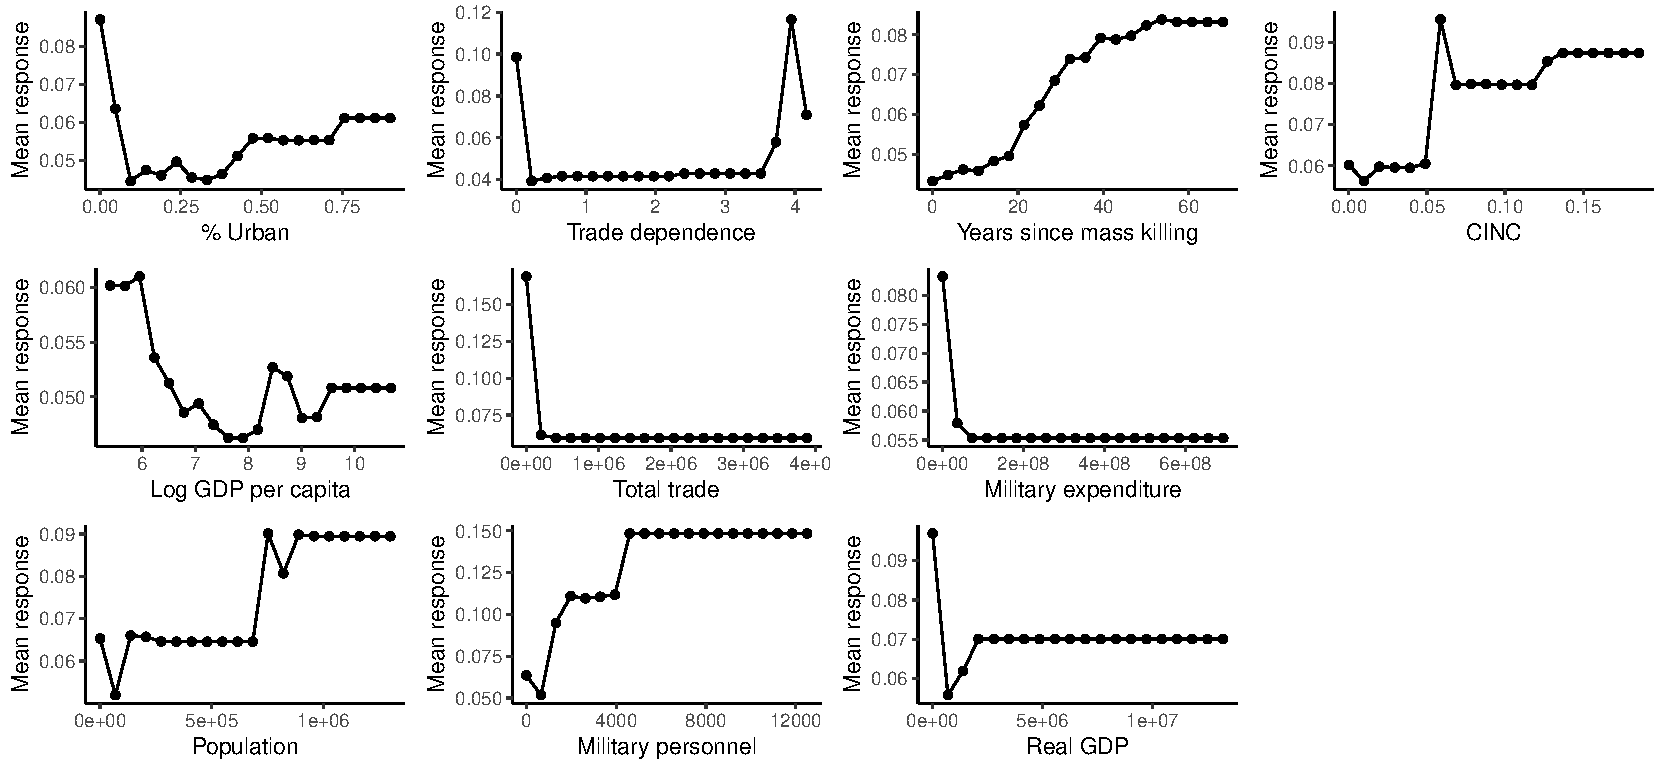
\includegraphics[width=\textwidth, height=8cm]{images/rf-ucdp-pd.pdf}
    \caption{Partial Dependence Plots -- Mass Killings during Civil Wars (UCDP Data)}
    \label{fig:drfdpp2}
\end{figure}
	
\begin{figure}[H]
    \begin{center}
    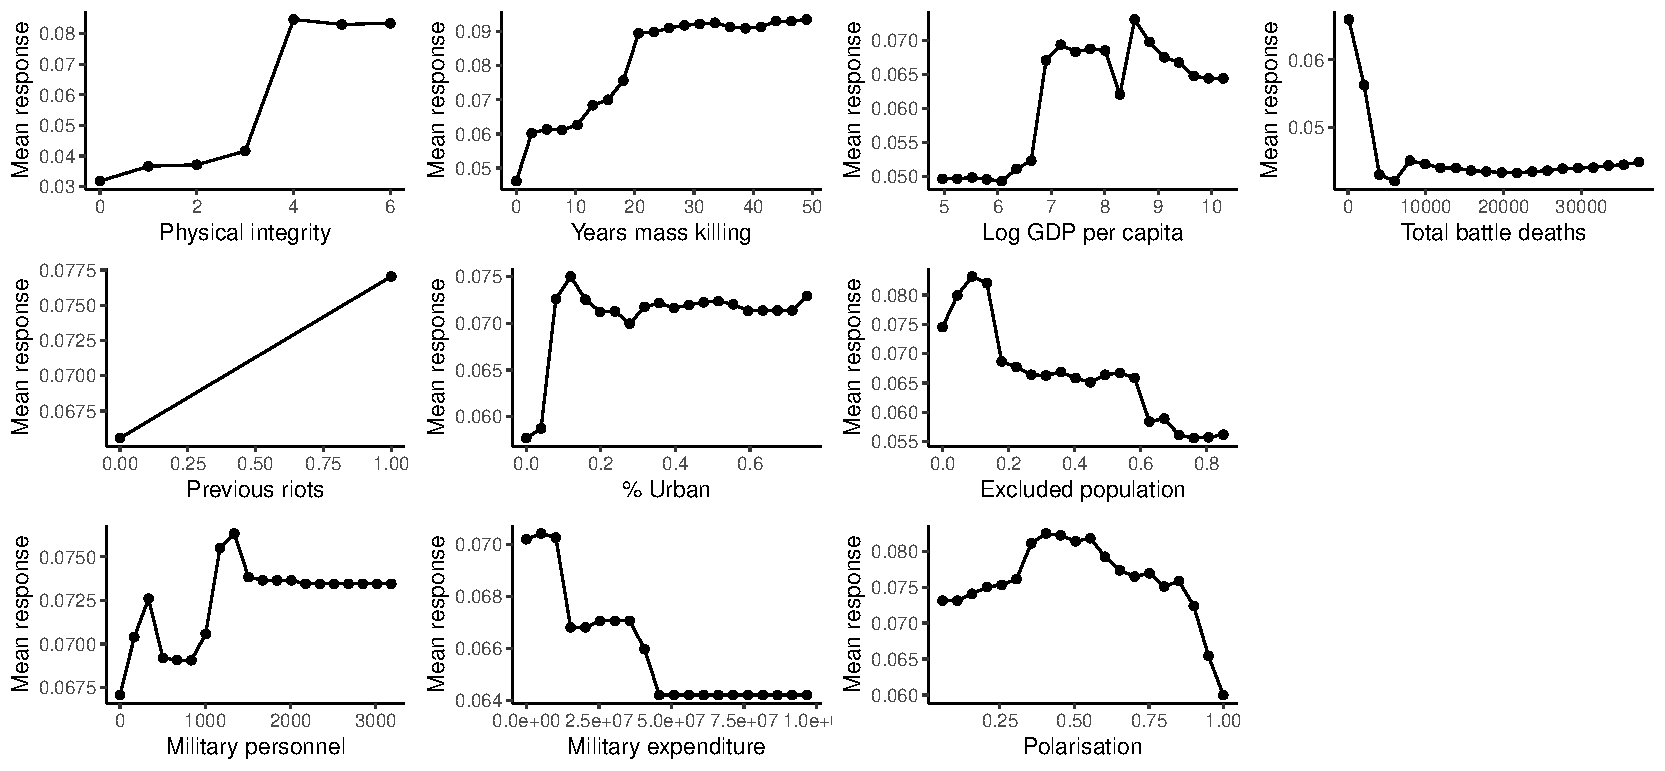
\includegraphics[width=\textwidth, height=8cm]{images/rf-cow-pd.pdf}
    \caption{Partial Dependence Plots -- Mass Killings during Civil Wars (COW Data)}
    \label{fig:drfdpp3}
    \end{center}
\end{figure}	
	
\begin{figure}[H]
    \begin{center}
    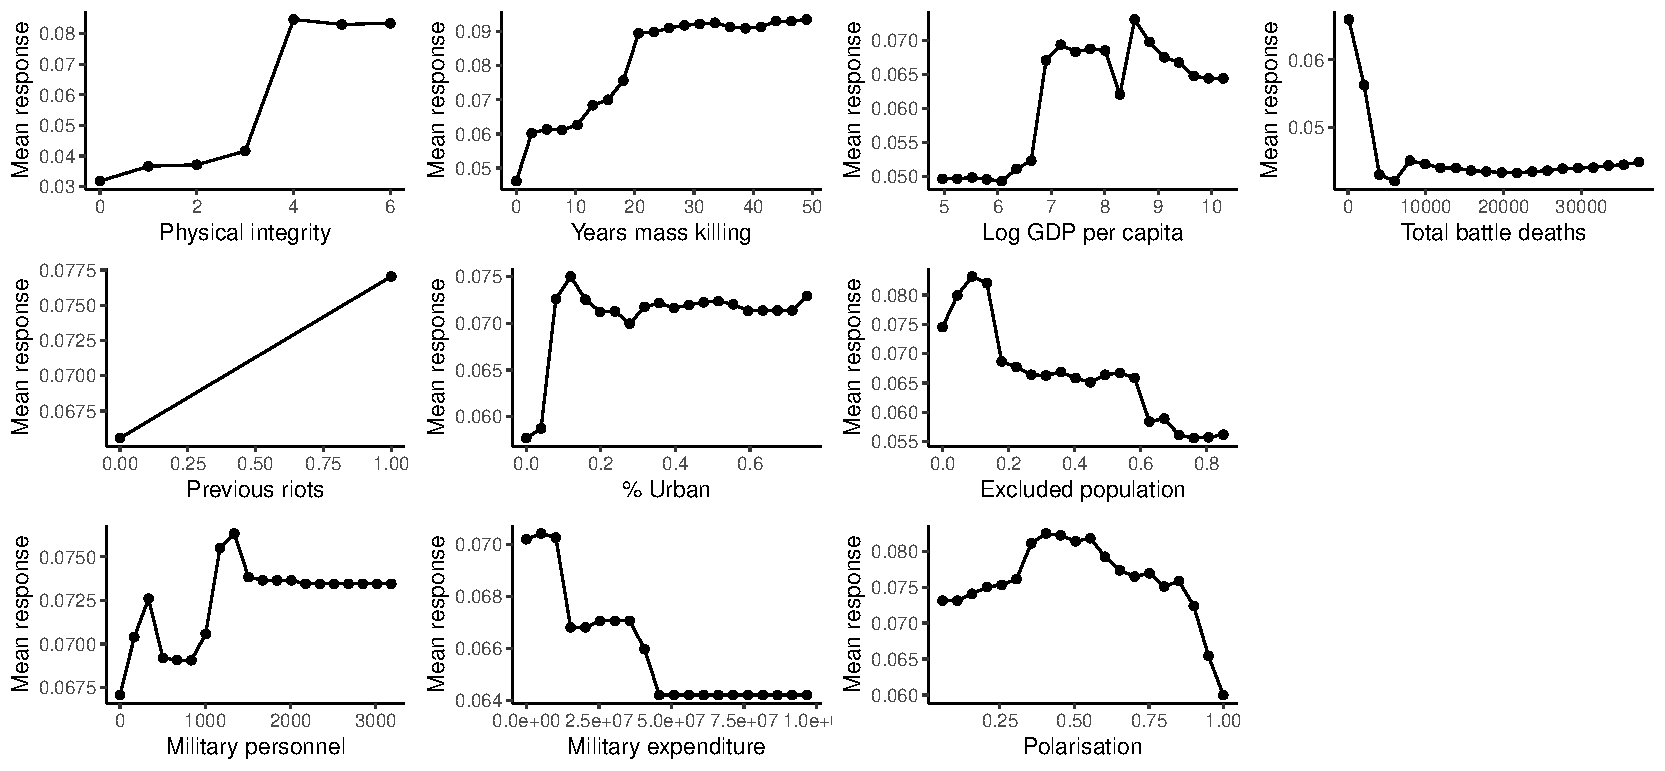
\includegraphics[width=\textwidth, height=8cm]{images/rf-cow-pd.pdf}
    \caption{Partial Dependence Plots -- Mass Killings during Civil Wars (Cederman et al. Data)}
    \label{fig:drfdpp4}
    \end{center}
\end{figure}
	
To answer Question 3,  we estimate the same regressions using Harff's (\citeyear{harff2003no}) indicator of genocide and politicide. We find that no variable appears significant in our EBA models for genocide or politicide onset in the full data set. When we limit our sample to civil war years, the Post-Cold War period is negatively correlated with the outcome when using the Correlates of War data set. Excluded population has a negative sign in more than 90\% of the models using both Correlates of War's and Cederman et al's (\citeyear{cederman2010ethnic}) indicators of conflict. Displaced population also has a negative effect in the Correlates of War data set. During ethnic conflicts, our dummy variable for political assassinations has a negative impact on the onset of genocides. Overall, from these EBA analyses, we conclude then that the significant covariates of genocide and politicide onset differ significantly from those of more general forms of government mass violence. Though, the opportunity story still receives some limited support in these models. However, the machine learning models using Harff's genocide and politicide data are comparable to the ones we present above, with a similar set of variables appearing in the random forest estimations. These results once more highlight that while the mass killing literature struggles to identify correlates of atrocity that are robust across model specification, scholars have done a much better job at identifying variables that help predict both the onset of genocide/politicide and mass killings, more broadly.
	
\section{Additional Tests}
\label{sec:additional-tests}
	
We estimate a set of additional regressions to assess the robustness of our main findings. In regard to EBA, we include 10 variants of our original model. They largely confirm our prior results. First, we varied the number of covariates included in each regression to 3 and 5 while keeping the $M$ set of 3 control variables. The results are the same as those of the main model, except that ethnic fractionalisation and Polity IV squared become marginally significant with a CDF(0) of about 0.88. Second, we place different restrictions on the variance inflation factor (VIF) to test whether multicollinearity is driving our results. The two models with different values of VIF are identical to the model reported here, while in the model with no VIF restriction ethnic fractionalisation again fails to meet our threshold by a very small margin. 
	
We also reestimate the models using logit and probit regressions. In order to deal with the issue of complete separation \citep{bell2015questioning,zorn2005solution} we follow \citet{gelman2008weakly} and add a weakly informative prior distribution to the coefficients. In both cases, the logarithm of GDP per capita, post-Cold War period, previous riots, and Polity IV squared remain significant. 
	
In regard to random forests, grid searches are themselves a data-driven selection of many possible machine learning models, thus it is not strictly necessary to run a batch of additional tests. Nevertheless, we performed a series of grid searches using three different seeds obtained from \href{https://random.org}{\texttt{http://random.org}} to estimate how different starting numbers influence the model outcomes. The output of those models are largely comparable.
	
The results of each of these analyses are available in online appendix.

\section{Conclusion}
\label{sec:conclusion}
	
In this paper, we apply extreme bounds analysis and distributed random forests to estimate the robustness and predictive ability of 40 variables that have been pointed out as potential determinants of mass killings. We find strong evidence that mass killings are unlikely to happen in rich, stable countries. Nevertheless, there is considerable heterogeneity in some of our results. The findings point out that mass killings have different causes according to the context in which they erupt, so a general theory of state atrocities may obscure important details in our understanding of state killings. Moreover, mass killings are rare events, so local factors likely play an important role in their onset \citep{straus2007second,straus2012destroy}.
	
Yet we see this diversity of outcomes under a positive light. Our results suggest new avenues for research, and we believe they also highlight the importance of scholars moving from simple cross-country regressions to methods that can yield more robust predictions. For instance, why are mass killings in ethnic conflicts correlated with a different set of variables than in armed conflicts in general? Would the results remain robust had scholars decided to code ethnic conflicts in another way? More theoretical advancement would also be welcome. Given that GDP per capita is negatively correlated to state atrocities in virtually every model, it would be interesting to unpack the causal mechanisms by which it operates by testing more specific mechanisms. 
	
In terms of practical implications, the results indicate that democratisation and pro-growth economic policies are the most efficient ways to prevent mass killings. The international community can therefore play a role in deterring leaders from using force against their own population, either by offering support for domestic opposition groups, intervening, or by fostering economic development. Although costly in the short run, and sometimes violent during the transition, these measures would substantially decrease the likelihood of state violence by breaking the ``conflict trap'' in which past conflicts create the condition for new ones \citep{collier2003breaking}.

\newpage
	
\bibliography{references}
\bibliographystyle{apalike}
\end{document}

